\section{Scope Management}
\label{sec:scope}
\lhead{\thesection \space Scope Management}
Scope management is what you do to make sure that your project includes all the work relevant to achieving the project’s objectives and not anything else. It’s about controlling what’s included in the project and what is not.

\subsection{Plan Scope Management}
This project is for designing, programming, and testing a new software product which will be a new module of the connected.football app to add a feature to vote on given exercises. This includes design of the software, all programming and coding, and testing/validation of the software.\\
For this project, scope management will be the sole responsibility of all group members. The scope for this project is defined by the Scope Statement, Work Breakdown Structure and the Software Requirement Specification. Proposed scope changes may be initiated by the product owner as well as every member of the team.

\begin{table}[H]
\centering
\begin{tabular}{|c|c|l|}
\hline

\cellcolor{gray}Name & 
\cellcolor{gray}Role &
\cellcolor{gray}Responsibilities \\\hline
Guido Bruzniak & Product owner &
- Approve or deny scope changes.\\&&
- Evaluate need for scope change requests.\\&&
- Accept project deliverables\\\hline
Lucas Gehlen&Team member&- Measure and verify project scope.\\
Marco Kull&&- Update project documents upon scope changes.\\
Patrick Richter&&- Measure and verify project scope.\\
Sebastian Wilczek&&- Participate in defining change resolutions.\\
&&- Evaluate the need for scope changes.\\\hline
\end{tabular}
\caption{Scope Roles \& Responsibilities}
\end{table}

\subsection{Collect Requirements}
The requirements for this project are delivered by the product owner. During the weekly meetings with the product owner the team will discuss the design fragments with him to ensure the requirements are met. All requirements will be documented in a software requirement specification document.
\subsection{Define Scope}
This project includes the design, programming, and testing of a new module of the connected.football app to add a feature to vote on given exercises. The deliverables for this project is a completed module with the flexibility to modify and expand as necessary in the future. This project will be accepted once the new module has been successfully tested. Assumptions for this project are that support will be provided by the project owner.
\subsection{Create WBS}

The project is broken down into three phases: Vote4Fun; Promotion Code; and Vote4Fun Group Extension. Each of these phases is then subdivided further down.
\begin{figure}[!ht]
	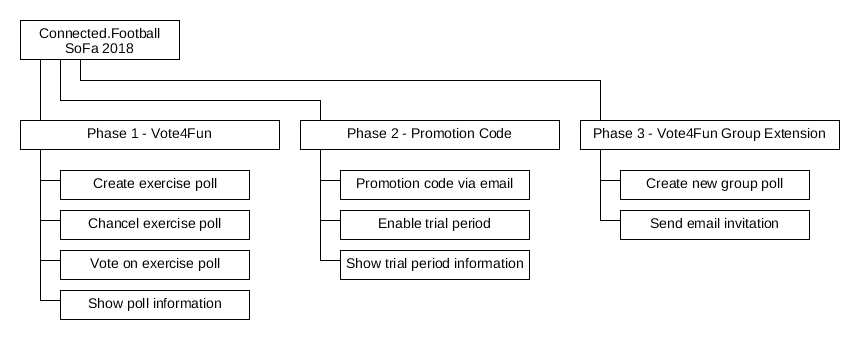
\includegraphics[width=\textwidth]{content/diagram/scope/wbs.png}
	\caption{Work Breakdown Structure}
\end{figure}
\subsection{Validate Scope}
As this project progresses the team will verify interim project deliverables against the original scope. To ensure that project work remains within the scope of the project those interim deliverables will be discussed in weekly meetings with the product owner.
\subsection{Control Scope}
The project team will work together to control of the scope of the project. The project manager will oversee the project team and the progression of the project to ensure that this scope control process if followed.\\
If a change to the project scope is needed, all team members and the product owner must approve of the scope change.